\documentclass{standalone}
\usepackage{tikz}
\usetikzlibrary{patterns, positioning}


\begin{document}
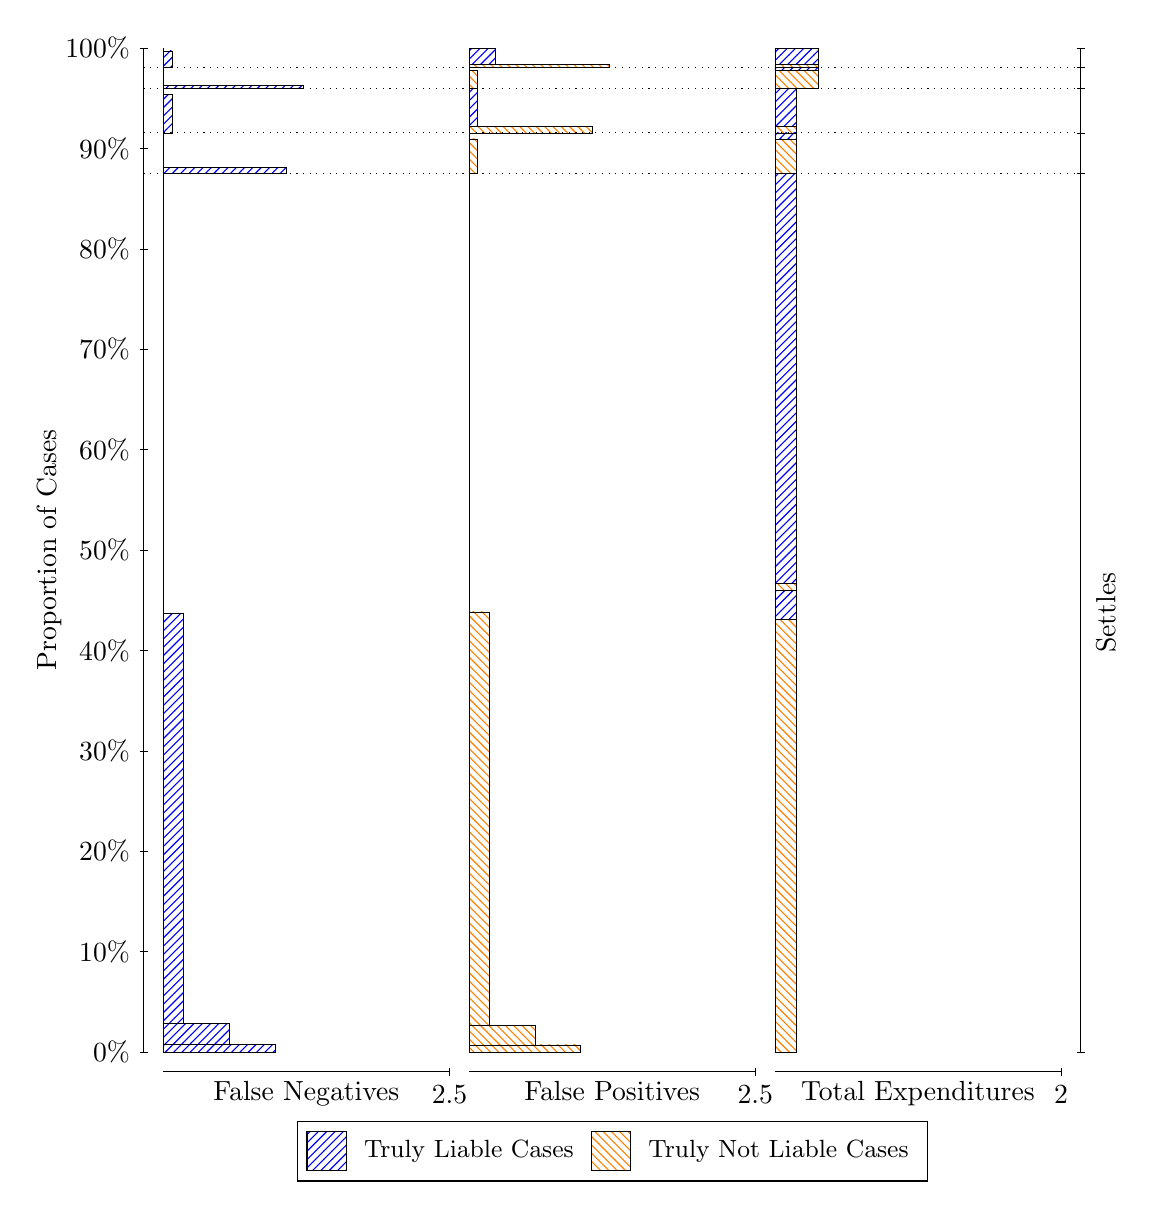
\begin{tikzpicture}
\draw[black, very thin] (1.5,1.75) -- (1.5,14.5);
\node[rotate=90, text=black, anchor=center] at (0.3, 8.125) {Proportion of Cases};
\draw[black, very thin] (1.45,1.75) -- (1.55,1.75);
\node[text=black, anchor=east] at (1.45, 1.75) {0\%};
\draw[black, very thin] (1.45,3.025) -- (1.55,3.025);
\node[text=black, anchor=east] at (1.45, 3.025) {10\%};
\draw[black, very thin] (1.45,4.3) -- (1.55,4.3);
\node[text=black, anchor=east] at (1.45, 4.3) {20\%};
\draw[black, very thin] (1.45,5.575) -- (1.55,5.575);
\node[text=black, anchor=east] at (1.45, 5.575) {30\%};
\draw[black, very thin] (1.45,6.85) -- (1.55,6.85);
\node[text=black, anchor=east] at (1.45, 6.85) {40\%};
\draw[black, very thin] (1.45,8.125) -- (1.55,8.125);
\node[text=black, anchor=east] at (1.45, 8.125) {50\%};
\draw[black, very thin] (1.45,9.4) -- (1.55,9.4);
\node[text=black, anchor=east] at (1.45, 9.4) {60\%};
\draw[black, very thin] (1.45,10.675) -- (1.55,10.675);
\node[text=black, anchor=east] at (1.45, 10.675) {70\%};
\draw[black, very thin] (1.45,11.95) -- (1.55,11.95);
\node[text=black, anchor=east] at (1.45, 11.95) {80\%};
\draw[black, very thin] (1.45,13.225) -- (1.55,13.225);
\node[text=black, anchor=east] at (1.45, 13.225) {90\%};
\draw[black, very thin] (1.45,14.5) -- (1.55,14.5);
\node[text=black, anchor=east] at (1.45, 14.5) {100\%};

\draw[black, very thin] (13.4,1.75) -- (13.4,14.5);
\draw[black, very thin] (13.35,1.75) -- (13.45,1.75);
\node[anchor=west] at (13.35, 1.75) {};
\draw[black, very thin] (13.35,12.908) -- (13.45,12.908);
\node[anchor=west] at (13.35, 12.908) {};
\draw[black, very thin] (13.35,13.422) -- (13.45,13.422);
\node[anchor=west] at (13.35, 13.422) {};
\draw[black, very thin] (13.35,13.991) -- (13.45,13.991);
\node[anchor=west] at (13.35, 13.991) {};
\draw[black, very thin] (13.35,14.254) -- (13.45,14.254);
\node[anchor=west] at (13.35, 14.254) {};
\draw[black, very thin] (13.35,14.5) -- (13.45,14.5);
\node[anchor=west] at (13.35, 14.5) {};

\draw[black, very thin, pattern color=blue, pattern=north east lines] (1.75,1.75) rectangle (3.167,1.848);
\draw[black, very thin, pattern color=blue, pattern=north east lines] (1.75,1.848) rectangle (2.5857,2.1121);
\draw[black, very thin, pattern color=blue, pattern=north east lines] (1.75,2.1121) rectangle (2.0043,7.3192);
\draw[black, very thin, pattern color=orange, pattern=north west lines] (1.75,7.3192) rectangle (1.75,12.908);
\draw[black, very thin, pattern color=blue, pattern=north east lines] (1.75,12.908) rectangle (3.3123,12.984);
\draw[black, very thin, pattern color=orange, pattern=north west lines] (1.75,12.984) rectangle (1.75,13.422);
\draw[black, very thin, pattern color=blue, pattern=north east lines] (1.75,13.422) rectangle (1.859,13.907);
\draw[black, very thin, pattern color=orange, pattern=north west lines] (1.75,13.907) rectangle (1.75,13.991);
\draw[black, very thin, pattern color=blue, pattern=north east lines] (1.75,13.991) rectangle (3.5303,14.025);
\draw[black, very thin, pattern color=orange, pattern=north west lines] (1.75,14.025) rectangle (1.75,14.254);
\draw[black, very thin, pattern color=blue, pattern=north east lines] (1.75,14.254) rectangle (1.859,14.464);
\draw[black, very thin, pattern color=orange, pattern=north west lines] (1.75,14.464) rectangle (1.75,14.5);
\draw[black, very thin, pattern color=orange, pattern=north west lines] (5.6333,1.75) rectangle (7.0503,1.8399);
\draw[black, very thin, pattern color=orange, pattern=north west lines] (5.6333,1.8399) rectangle (6.469,2.0845);
\draw[black, very thin, pattern color=orange, pattern=north west lines] (5.6333,2.0845) rectangle (5.8877,7.3386);
\draw[black, very thin, pattern color=blue, pattern=north east lines] (5.6333,7.3386) rectangle (5.6333,12.908);
\draw[black, very thin, pattern color=orange, pattern=north west lines] (5.6333,12.908) rectangle (5.7423,13.346);
\draw[black, very thin, pattern color=blue, pattern=north east lines] (5.6333,13.346) rectangle (5.6333,13.422);
\draw[black, very thin, pattern color=orange, pattern=north west lines] (5.6333,13.422) rectangle (7.1957,13.506);
\draw[black, very thin, pattern color=blue, pattern=north east lines] (5.6333,13.506) rectangle (5.7423,13.991);
\draw[black, very thin, pattern color=orange, pattern=north west lines] (5.6333,13.991) rectangle (5.7423,14.22);
\draw[black, very thin, pattern color=blue, pattern=north east lines] (5.6333,14.22) rectangle (5.6333,14.254);
\draw[black, very thin, pattern color=orange, pattern=north west lines] (5.6333,14.254) rectangle (7.4137,14.289);
\draw[black, very thin, pattern color=blue, pattern=north east lines] (5.6333,14.289) rectangle (5.9603,14.5);
\draw[black, very thin, pattern color=orange, pattern=north west lines] (9.5167,1.75) rectangle (9.7892,7.2487);
\draw[black, very thin, pattern color=blue, pattern=north east lines] (9.5167,7.2487) rectangle (9.7892,7.6108);
\draw[black, very thin, pattern color=orange, pattern=north west lines] (9.5167,7.6108) rectangle (9.7892,7.7007);
\draw[black, very thin, pattern color=blue, pattern=north east lines] (9.5167,7.7007) rectangle (9.7892,12.908);
\draw[black, very thin, pattern color=orange, pattern=north west lines] (9.5167,12.908) rectangle (9.7892,13.346);
\draw[black, very thin, pattern color=blue, pattern=north east lines] (9.5167,13.346) rectangle (9.7892,13.422);
\draw[black, very thin, pattern color=orange, pattern=north west lines] (9.5167,13.422) rectangle (9.7892,13.506);
\draw[black, very thin, pattern color=blue, pattern=north east lines] (9.5167,13.506) rectangle (9.7892,13.991);
\draw[black, very thin, pattern color=orange, pattern=north west lines] (9.5167,13.991) rectangle (10.062,14.22);
\draw[black, very thin, pattern color=blue, pattern=north east lines] (9.5167,14.22) rectangle (10.062,14.254);
\draw[black, very thin, pattern color=orange, pattern=north west lines] (9.5167,14.254) rectangle (10.062,14.289);
\draw[black, very thin, pattern color=blue, pattern=north east lines] (9.5167,14.289) rectangle (10.062,14.5);
\draw[black, dotted] (1.5,12.908) -- (13.4,12.908);
\draw[black, dotted] (1.5,13.422) -- (13.4,13.422);
\draw[black, dotted] (1.5,13.991) -- (13.4,13.991);
\draw[black, dotted] (1.5,14.254) -- (13.4,14.254);
\draw[black, very thin] (1.75,1.5) -- (5.3833,1.5);
\node[text=black, anchor=north] at (3.5667, 1.5) {False Negatives};
\draw[black, very thin] (5.3833,1.45) -- (5.3833,1.55);
\node[text=black, anchor=north] at (5.3833, 1.45) {2.5};

\draw[black, very thin] (5.6333,1.5) -- (9.2667,1.5);
\node[text=black, anchor=north] at (7.45, 1.5) {False Positives};
\draw[black, very thin] (9.2667,1.45) -- (9.2667,1.55);
\node[text=black, anchor=north] at (9.2667, 1.45) {2.5};

\draw[black, very thin] (9.5167,1.5) -- (13.15,1.5);
\node[text=black, anchor=north] at (11.333, 1.5) {Total Expenditures};
\draw[black, very thin] (13.15,1.45) -- (13.15,1.55);
\node[text=black, anchor=north] at (13.15, 1.45) {2};

\node[text=black, centered, rotate=90] at (13.72, 7.3289) {Settles};





\draw (7.449999999999999,1.5) node[draw=none] (baseCoordinate) {};
\begin{scope}[align=center]
        \matrix[scale=0.5, draw=black, below=0.5cm of baseCoordinate, nodes={draw}, column sep=0.1cm]{
            \node[rectangle, draw, minimum width=0.5cm, minimum height=0.5cm, pattern color=blue, pattern=north east lines] {}; &
            \node[draw=none, font=\small, text=black] (B) {Truly Liable Cases}; &
            \node[rectangle, draw, minimum width=0.5cm, minimum height=0.5cm, pattern color=orange, pattern=north west lines] {}; &
            \node[draw=none, font=\small, text=black] (B) {Truly Not Liable Cases}; \\
            };
\end{scope}

\end{tikzpicture}
\end{document}